\documentclass[UTF8]{article}
\usepackage[UTF8]{ctex}

%----------- 版式与字体 ----------------
\usepackage{geometry}
\geometry{a4paper,margin=2.5cm}
\setlength{\parindent}{2em}
\setlength{\parskip}{0.5em}
\renewcommand{\baselinestretch}{1.3}

%----------- 列表与颜色 ----------------
\usepackage[shortlabels]{enumitem}
\setlist[enumerate]{label=\arabic*.}
\usepackage{xcolor}
\usepackage{titlesec}

%----------- 数学宏包 ------------------
\usepackage{amsmath}
\usepackage{amsfonts}
\usepackage{amssymb}

% 添加必要的宏包
\usepackage{graphicx} % 支持插入图片
\usepackage{subcaption} % 支持子图
\usepackage{float} % 支持H选项
\usepackage{siunitx}
\usepackage{listings}
\usepackage{url} % 支持\url命令
\usepackage{tikz} % 支持tikzpicture环境
\usetikzlibrary{positioning} % 支持right=of语法
\usetikzlibrary{decorations.pathreplacing} % 支持brace装饰
\lstset{language=Python, basicstyle=\ttfamily\footnotesize, showstringspaces=false, tabsize=4}


%----------- 题注样式(节标题) ---------
\titleformat{\section}
  {\zihao{4}\bfseries}{\chinese{section}、}{0.5em}{}
\titleformat{\subsection}
  {\zihao{5}\bfseries}{\arabic{section}.\arabic{subsection}}{0.5em}{}

%----------- 正文开始 ------------------
\begin{document}

\begin{center}
  {\zihao{3}\bfseries 人工智能实验报告}\\[1ex]
  {\zihao{4} 实验4\quad 综合实验}
\end{center}

% ----------- 信息栏 -------------------
\renewcommand{\arraystretch}{1.6}
\begin{tabular}{p{5cm}p{5.5cm}p{3cm}p{5.5cm}}
  学院:计算机与通信工程 & 专业:计算机科学与技术 & 班级:计221\\
  姓名:乔彦博 & 学号:U202242223 & 日期:2025.5.9\\
\end{tabular}

\section{实验内容}

\subsection{实验目标与任务背景}

人体动作识别是计算机视觉领域的重要研究方向之一,在智能监控、人机交互等应用中具有广泛的需求。本实验旨在利用3D骨架序列数据实现对人体动作类别的自动识别分类。骨架序列由人体各关键关节的三维坐标随时间变化构成,能够有效表示人体的动态姿态特征且不受光照、背景等环境因素影响,因此成为动作识别研究的有效表征方式之一。基于此,本实验选择了以CSV文件格式存储的3D骨架数据作为输入,构建并训练深度学习模型以完成对给定序列所对应动作类别的预测。

\subsection{数据处理流程}

在数据预处理中,我们需要将原始骨架序列CSV文件转换为模型可以接受的输入格式。每个CSV文件包含了一段动作的骨架运动序列,其中每一行记录了该序列中某一帧的人体所有关节坐标值(例如,各关节的$x, y, z$坐标)。通过逐行读取CSV文件,可以依次重建出动作的时间序列关节数据。由于不同序列的帧数可能不同,为方便批量训练,我们对序列进行了长度对齐:针对短于预定长度的序列在末尾填充默认值(例如零值)帧,即进行\textbf{padding}操作,使所有序列长度一致。同时,我们从文件名中提取该序列对应的动作标签。例如,文件名中包含的``action001''字段可映射为动作类别标签1号。最后,经过读取、填充等处理后,我们得到规范化的“骨架序列+标签”样本数据,用于后续模型训练(如图\ref{fig:process}所示)。

\begin{figure}[htbp]
    \centering
    \begin{tikzpicture}[node distance=1.8cm, align=center]
        \node[draw, rectangle] (csv) {骨架CSV文件};
        \node[draw, rectangle, right=of csv, text width=1cm] (read) {逐帧读取\\3D关节坐标序列};
        \node[draw, rectangle, right=of read, text width=1cm] (pad) {序列填充\\(Padding)};
        \node[draw, rectangle, right=of pad, text width=1cm] (label) {提取标签\\(动作类别)};
        \node[draw, rectangle, right=of label, text width=1cm] (dataset) {训练样本\\(序列+标签)};
        \draw[->, thick] (csv) -- (read);
        \draw[->, thick] (read) -- (pad);
        \draw[->, thick] (pad) -- (label);
        \draw[->, thick] (label) -- (dataset);
    \end{tikzpicture}
    \caption{骨架数据预处理流程:从CSV文件逐帧读取骨架序列,经过填充处理得到统一长度的序列,并提取对应的动作标签形成训练样本。}
    \label{fig:process}
\end{figure}

\subsection{模型结构}

本实验采用了\textbf{BiLSTM+Attention}的神经网络模型结构,如图\ref{fig:model}所示。首先,利用双向长短期记忆网络(BiLSTM)对输入的骨架序列进行时序特征提取。BiLSTM由正向和反向两个LSTM组成,能够同时从过去和未来两个方向建模时间依赖关系,从而获得每个时间步的综合隐藏表示$\mathbf{h}_t$(包含了序列在该时刻前后的信息)。

随后,我们引入\textbf{注意力机制(Attention)}对BiLSTM产生的隐藏状态序列$\{\mathbf{h}_1, \mathbf{h}_2, \dots, \mathbf{h}_T\}$进行加权融合。具体来说,注意力层为每个时间步的隐藏向量$\mathbf{h}_t$分配一个权重系数$\alpha_t$(通过与可学习的上下文向量计算相关性得到),并对隐藏向量进行加权求和得到\textbf{上下文向量}$\mathbf{c}=\sum_{t=1}^{T} \alpha_t \mathbf{h}_t$。权重$\alpha_t$反映了时刻$t$对最终动作判别的相对重要性,从而使模型能够自适应地关注对区分动作最关键的那些帧。最后,将得到的上下文向量$\mathbf{c}$传入全连接输出层,经过Softmax激活,生成各动作类别的预测概率分布。模型判定概率最高的类别为输入序列的识别结果。

\begin{figure}[htbp]
    \centering
    \begin{tikzpicture}[node distance=1.4cm and 1.5cm, >=stealth, font=\small]
        % BiLSTM输出序列
        \node[draw, circle, fill=blue!7, minimum size=1.1cm] (h1) {$h_1$};
        \node[draw, circle, fill=blue!7, below=1cm of h1] (h2) {$h_2$};
        \node[draw, circle, fill=blue!7, below=1cm of h2] (h3) {$h_3$};

        % Attention汇聚
        \node[draw, circle, fill=orange!18, right=1.5cm of h2, minimum size=1.4cm, font=\normalsize, align=center] (attn) {$\sum$\\Attention};

        % 输出层
        \node[draw, rectangle, fill=green!12, right=2.0cm of attn, minimum width=2.3cm, minimum height=0.9cm, align=center] (out) {输出层\\(Softmax)};

        % 箭头与权重
        \draw[->, thick] (h1.east) -- node[above,pos=0.60] {$\alpha_1$} (attn.140);
        \draw[->, thick] (h2.east) -- node[above,pos=0.55] {$\alpha_2$} (attn.180);
        \draw[->, thick] (h3.east) -- node[below,pos=0.60] {$\alpha_3$} (attn.220);

        % Attention输出
        \draw[->, thick] (attn) -- node[above] {上下文向量 $c$} (out);

        % 输出层到最终预测
        \node[right=1.5cm of out, font=\normalsize] (class) {动作类别预测};
        \draw[->, thick] (out) -- (class);

        % Brace & 输入标签
        \draw[decorate, decoration={brace, amplitude=5pt}, thick]
          ([yshift=8pt]h1.north west) -- ([yshift=-8pt]h3.south west)
            node[midway, left=8pt, align=center, font=\normalsize, rotate=90] {BiLSTM\\隐藏状态序列};
        \node[left=1.8cm of h2, font=\normalsize] (input) {输入骨架序列};

        % 虚线输入
        \draw[->, dashed, thick] (input) -- (h2.west);

    \end{tikzpicture}
    \caption{BiLSTM+Attention模型结构示意图:输入骨架序列经BiLSTM提取为隐藏状态序列$\{h_t\}$,Attention按权重$\alpha_t$汇聚为上下文向量$c$,最后经Softmax输出类别预测。}
    \label{fig:model}
\end{figure}


\subsection{核心代码与结构解析}

\vspace{0.5em}
\noindent
\textbf{模型代码(Python):}
\begin{lstlisting}[language=Python, caption={BiLSTM+Attention模型主结构}]
class ActionClassifier(nn.Module):
    def __init__(self, input_dim, hidden_dim=256, num_layers=2, num_classes=8, dropout=0.3):
        super().__init__()
        self.lstm = nn.LSTM(
            input_size   = input_dim,
            hidden_size  = hidden_dim,
            num_layers   = num_layers,
            batch_first  = True,
            bidirectional= True,
            dropout      = dropout if num_layers > 1 else 0.0)
        self.attn_pool = AttentionPooling(hidden_dim * 2)
        self.fc = nn.Sequential(
            nn.Linear(hidden_dim * 2, hidden_dim),
            nn.ReLU(),
            nn.Dropout(dropout),
            nn.Linear(hidden_dim, num_classes)
        )

    def forward(self, x):
        h, _ = self.lstm(x)            # LSTM时序特征
        context = self.attn_pool(h)    # 注意力池化
        logits = self.fc(context)      # 分类输出
        return logits

class AttentionPooling(nn.Module):
    def __init__(self, hidden_dim):
        super().__init__()
        self.score = nn.Linear(hidden_dim, 1, bias=False)
    def forward(self, h):              # h: (B, T, H)
        α = torch.softmax(self.score(h).squeeze(-1), dim=1)  # (B, T)
        return torch.sum(h * α.unsqueeze(-1), dim=1)         # (B, H)
\end{lstlisting}

\vspace{0.5em}
\noindent
\textbf{结构:}
\begin{enumerate}
    \item \textbf{输入层:} 采集到的骨架序列被处理成$\mathrm{[batch, T, F]}$格式,其中$T$为时序长度,$F$为每帧特征维数。
    \item \textbf{BiLSTM:} 用于提取序列双向时序特征。每一帧都由正向与反向LSTM综合编码,输出序列$\mathbf{H}=(h_1,\dots,h_T)$。
    \item \textbf{AttentionPooling:} 对BiLSTM所有时刻的隐藏状态按“重要性”加权,自动聚焦关键帧,输出整个序列的上下文表示$c$。
    \item \textbf{全连接+Dropout:} 进一步非线性变换与正则化,最后输出$\mathrm{num\_classes}$维的分类概率。
\end{enumerate}

\section{实验过程}

\subsection{训练集和测试集的构造}

在模型训练前,我们首先构造了训练集和测试集,用于模型学习和性能评估。具体地,将全部动作序列样本按照约\textbf{9:1}的比例随机划分为训练集和测试集。在划分时保证各类动作在训练和测试中都有分布,以防止某一类别仅出现在测试集从而无法被模型学到。由于原始数据的动作标签采用非连续编号(例如``001''表示某一动作类别),因此我们对标签进行了重新编码映射,使之成为从0开始的连续整数标签,便于模型输出和计算损失时的处理(例如,将``action001''映射为类别0)。完成上述处理后,训练集中包含了绝大部分样本用于模型参数学习,测试集的样本将仅用于在训练完成后评估模型的泛化表现。

\subsection{模型训练过程}

在训练阶段,我们采用交叉熵作为损失函数,选用Adam优化器(学习率0.001)来更新模型参数。训练过程中每批次输入一个批量的序列样本(例如批量大小16),模型的参数根据损失梯度不断更新。本实验训练迭代了若干个epoch(例如50轮),直到模型在训练集上的性能收敛。训练过程中,我们记录了每个epoch的损失值(Loss)以及在训练集上的准确率(Accuracy),并绘制成曲线图以观察模型的收敛情况。如图\ref{fig:train}所示,Loss曲线随着训练迭代次数的增加持续下降,而准确率曲线则不断上升并逐渐趋于平稳。这表明模型在逐步学习骨架序列与动作类别之间的对应关系,训练收敛效果良好。

\begin{figure}[htbp]
    \centering
    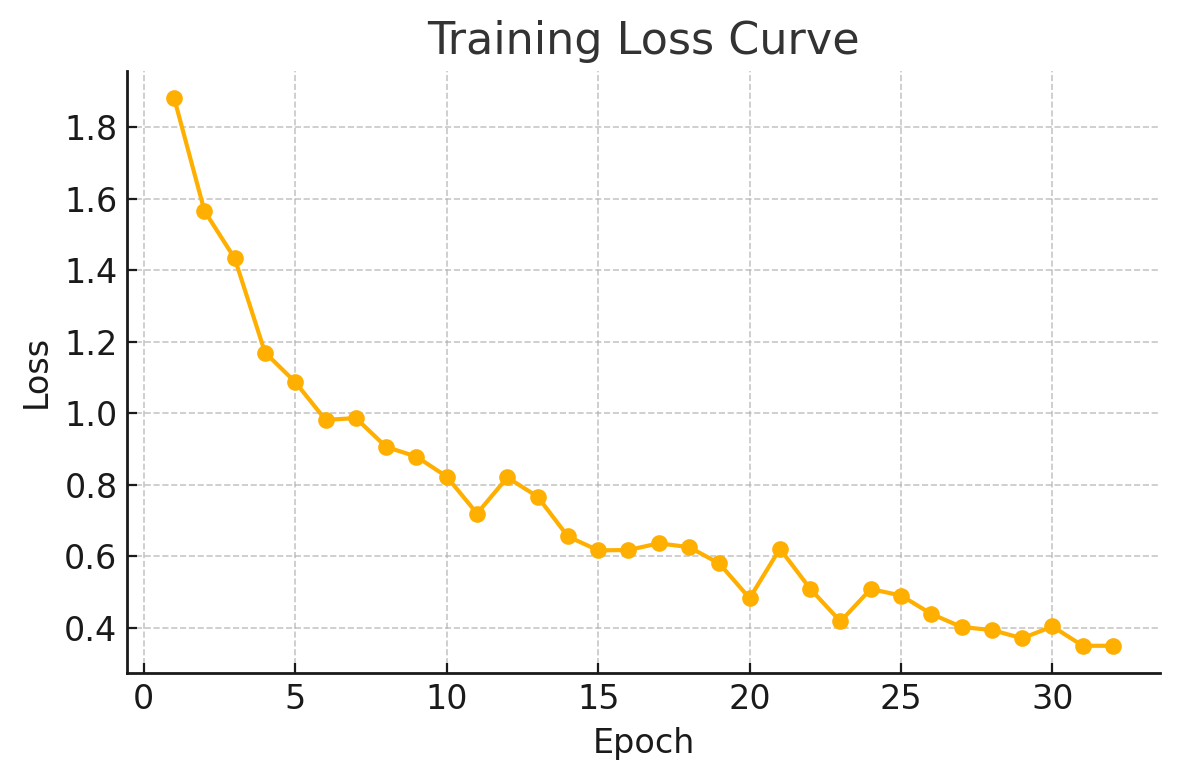
\includegraphics[width=0.45\textwidth]{loss_curve.png}
    \quad
    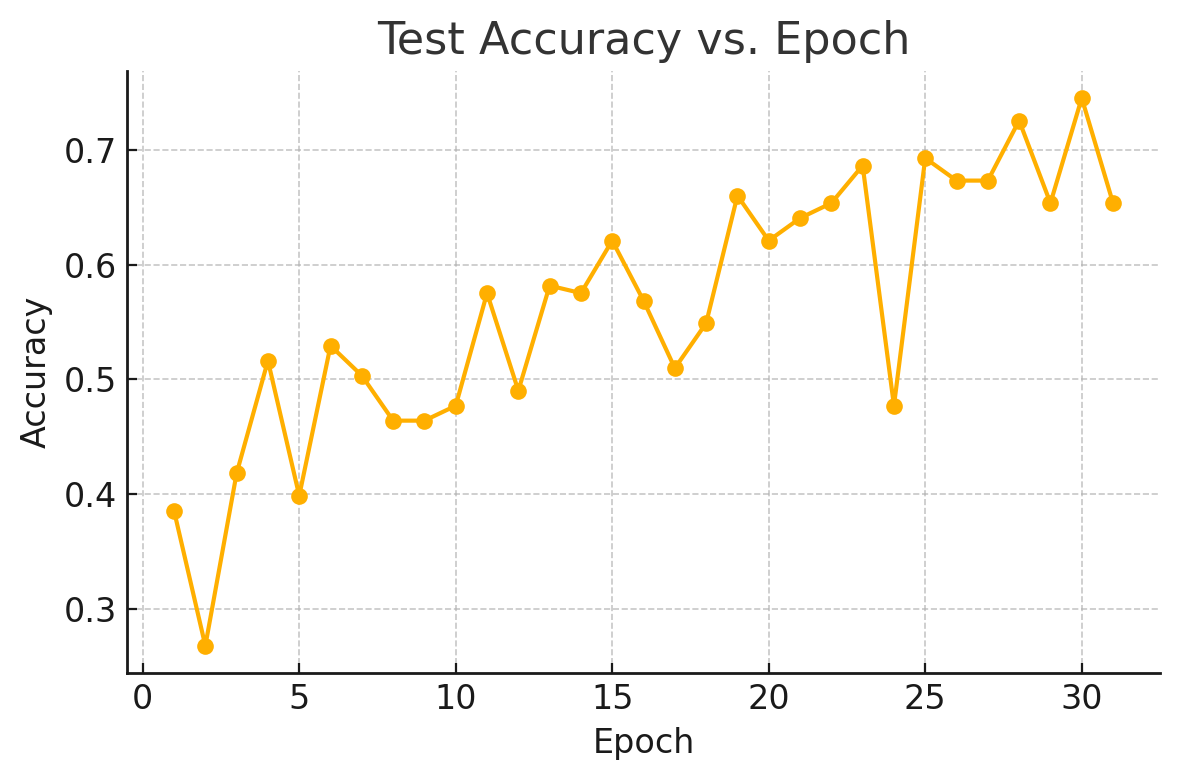
\includegraphics[width=0.45\textwidth]{acc_curve.png}
    \caption{模型训练过程中Loss和Accuracy变化曲线。(左)训练损失值随epoch的下降趋势;(右)训练准确率随epoch的上升趋势。}
    \label{fig:train}
\end{figure}

\subsection{测试与结果可视化}

模型训练完成后,我们使用\textbf{测试集}的数据对模型进行了性能评估。首先,利用训练好的模型对测试集中每个序列样本进行预测,得到其预测的动作类别,与真实标签进行对比,计算模型的整体分类指标。同时,我们绘制了模型在测试集上的\textbf{混淆矩阵}和\textbf{ROC曲线}以直观展示分类效果(见图\ref{fig:results})。图\ref{fig:results}左侧给出了混淆矩阵,其中行表示真实类别,列表示模型预测类别,矩阵中的数值代表对应真实-预测组合的样本数量。理想情况下,混淆矩阵应接近对角矩阵形式(只有对角线元素为大值),图中可以看到多数样本被正确分类在对角线位置,但某些类别存在被误分类的情况。图\ref{fig:results}右侧展示了各动作类别对应的ROC曲线(采用一对多分类方式计算得到)。ROC曲线越靠近左上角表示分类性能越好。可以看出,对于大部分动作类别,模型的ROC曲线都较为陡峭,显示出较高的真阳性率和较低的假阳性率,表明模型能够较好地区分这些动作;而对于个别容易混淆的动作,其ROC曲线偏向对角线,反映出模型区分该类动作的能力有限。

\begin{figure}[htbp]
    \centering
    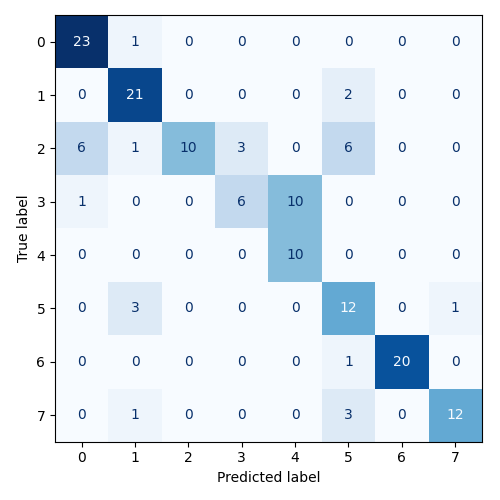
\includegraphics[width=0.45\textwidth]{confusion_matrix.png}
    \quad
    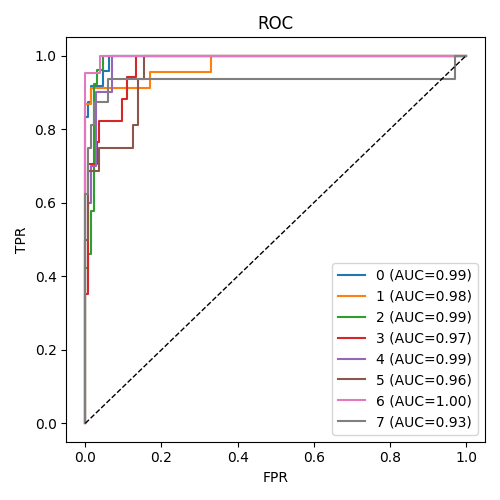
\includegraphics[width=0.45\textwidth]{roc_curves.png}
    \caption{模型在测试集上的分类结果可视化。(左)混淆矩阵:横轴为模型预测类别,纵轴为真实类别;(右)各类别动作的ROC曲线。}
    \label{fig:results}
\end{figure}

\section{实验结果分析}

综合测试结果评估,模型在测试集上取得了约\textbf{0.7450}的整体准确率(Accuracy)。同时,我们计算了Precision、Recall和F1-Score等评价指标,分别达到约\textbf{0.7500}、\textbf{0.7320}和\textbf{0.7405}。这些指标反映了模型对各类别动作的平均分类性能。

从混淆矩阵可以进一步观察各个动作类别的分类情况。总体来看,大部分动作能够被模型正确识别,其中某些动作的识别精度最高(例如类别3的所有测试样本几乎均被正确分类),说明该类动作的骨架运动特征较为鲜明,不易与其他动作混淆。而少数动作的识别效果较差,在测试集中经常被误分类为其他类别。例如,动作7往往被错认成与其运动模式相似的动作6,这导致该类别的召回率偏低。产生这种现象的原因可能是这些动作在骨架序列上的运动轨迹过于相近,模型难以提取区分二者的关键特征。

此外,本次实验所用的模型和方法仍存在一些\textbf{局限性}:(1) 对于动作持续时间或快慢节奏的变化(即\textbf{时序变形}),模型的鲁棒性有待提高。如果同一动作执行得过快或过慢,序列帧分布发生变化,当前模型可能无法充分适应这种变动,从而影响分类准确率。(2) 模型仅基于关节坐标序列进行学习,没有显式利用人体骨架各关节之间的拓扑结构关系。当不同动作在空间运动模式上存在部分相似时,这种缺乏先验结构的信息可能使模型难以区分动作细节。(3) 在训练样本数量有限的情况下,深度模型容易出现\textbf{过拟合}现象,即在训练集上表现良好但在新样本上泛化性能不足。这提示我们可能需要更多的数据、正则化技术或更简单的模型来缓解过拟合问题。

\section{实验总结与拓展研究}

通过本次综合实验,我们熟悉了\textbf{基于骨架序列的数据处理与动作识别}的完整流程,掌握了将原始CSV数据转换为模型输入、构建并训练序列深度学习模型以及评估模型性能的方法。我们体会到,引入\textbf{注意力机制}能够有效提升模型对关键时序信息的捕捉,从而提高动作分类的准确率。本实验所实现的BiLSTM+Attention模型在测试集上取得了一定的效果,但也暴露出模型在处理某些复杂动作时的不足。

针对\textbf{实时动作识别}应用,仍有诸多挑战需要应对。实时系统要求模型能够在动作发生过程中尽早给出判断,而不必等待整个动作完成,这就要求算法具有低延迟的响应能力。为此,可以采用\textbf{滑动窗口}的方法对连续到达的骨架帧进行在线识别:将最近固定长度的帧组成序列输入模型,当有新帧进入时滑动窗口向前移动并更新模型输出,从而实现对正在进行动作的动态检测。此外,需要对模型进行优化以降低每次推理的时间开销。初步方案包括模型压缩(例如剪枝、量化)、采用更高效的轻量级模型结构,以及充分利用GPU等硬件加速,以确保在实时场景下模型的推理延迟足够低,不影响系统的及时响应。

在后续的拓展研究中,我们可以考虑引入更先进的模型来提升动作识别的性能和鲁棒性。例如,将\textbf{图卷积网络(GCN)}应用于骨架数据以显式建模关节之间的连接关系,或采用基于Transformer的时序建模方法来捕获更长距离的时序依赖。这些方向都有望进一步提高对复杂动作的识别效果,并增强模型对时序变形和个体差异的鲁棒性。

\end{document}